\documentclass[review,5p,twocolumn,sort&compress,times]{elsarticle}

\usepackage{lineno}
% \usepackage{hyperref}

%%%%%% SYMBOLES %%%%%
\usepackage{tipa}	% pour avoir l'accent concave
\usepackage{lmodern}	% pour les guillemets
\usepackage{nth}	% pour ^th près des chiffres

%%%%%% EQUATION %%%%%%
\usepackage{amssymb}
\usepackage{amsmath}
\usepackage{fancybox}
\usepackage{xfrac}	% fraction de type "1/4"
\usepackage[fleqn]{cases}	% système équation
\usepackage[overload]{empheq}
\usepackage{bm}		% pour mettre en gras .
\usepackage{units} 	% x/y barre latérale pour les fractions
%\usepackage{split}

%%%%%% FIGURE %%%%%%
\usepackage{graphicx}	% insérer des graphiques
\usepackage{float}	% utiliser H dans les figures
\usepackage{subcaption}


%%%%%% TABLEAUX %%%%%%
\usepackage{array,multirow,makecell}
\usepackage[table,xcdraw]{xcolor} % pour avoir des lignes colorées dans les tableau
\usepackage{hhline}	% pour les lignes horizontales
\usepackage{tabularx} % permet itemize dans les cellules
\usepackage{booktabs}

\newcolumntype{L}[1]{>{\raggedright\let\newline\\\arraybackslash\hspace{0pt}}m{#1}}
\newcolumntype{C}[1]{>{\centering\let\newline\\\arraybackslash\hspace{0pt}}m{#1}}
\newcolumntype{R}[1]{>{\raggedleft\let\newline\\\arraybackslash\hspace{0pt}}m{#1}}

%%%%%%%%%%%%%%%%%%%%%
\usepackage{url}	% gérer les adresses www.

\newcommand{\ml}[1]{\textcolor{red}{ML : #1}}
\modulolinenumbers[5]

\begin{document}

\begin{frontmatter}

\title{Road traffic sound level estimation from realistic urban sound mixtures by Non-negative Matrix Factorization}

\author[ifsttar]{Jean-R\'emy Gloaguen\corref{cor1}}
\ead{jean-remy.gloaguen@ifsttar.fr}
\author[ifsttar]{Arnaud Can}
\author[ls2n]{Mathieu Lagrange}
\author[ls2n]{Jean-Fran\c cois Petiot}

\cortext[cor1]{Corresponding author}
\address[ifsttar]{Ifsttar Centre de Nantes, UMRAE, All\'ee des Ponts et Chauss\'es, 44344 Bouguenais, France}
\address[ls2n]{LS2N, 1 rue de No\"e, 44331 Nantes, France}

\begin{abstract}

Experimental acoustic sensor networks are currently tested in large cities, and appear more and more as a useful tool to enrich modeled road traffic noise maps through data assimilation techniques. One challenge is to be able to isolate from the measured sound mixtures acoustic quantities of interest such as the  sound level of road traffic. This task is anything but trivial because of the multiple sound sources that overlap within urban sound mixtures.

In this paper, the Non-negative Matrix Factorization (NMF) framework is developed to estimate road traffic noise levels within urban sound scenes. To evaluate the performances of the proposed approach, a synthetic corpus of sound scenes is designed, to cover most common soundscape settings, and whom realism is validated through a perceptual test. The simulated scenes reproduce then the sensor network outputs, in which the actual occurrence and sound level of each source are known.

Several variants of NMF are tested. The proposed approach, named threshold initialized NMF, appears to be the most reliable approach, allowing road traffic noise level estimation with average errors of less than 1.3 dB over the tested corpus of sound scenes.

\end{abstract}

\begin{keyword}
Non-negative Matrix Factorization \sep urban sound environment \sep road traffic sound level estimation
\end{keyword}

\end{frontmatter}

\linenumbers

\section{Introduction}

In response to the growing demand from urban dwellers for a better environment, noise mapping has been recommended as a tool to tackle noise pollution. The enactment of the European Directive 2002/EC/49 makes such maps mandatory to cities over 100 000 inhabitants. Those maps play an important informative role, establishing the distribution of the sound levels all over the cities as well as the estimation of the number of city dwellers exposed to high sound level ($>$ 55 dB(A)) \cite{nugent2014noise}. Road traffic concentrates particular attention as it is the main urban source of noise annoyance. Road traffic noise maps are typically built from data collection that consist of traffic data collected on the main roads (flow rates, mean speeds and heavy vehicle ratio) and urban geographic data (building heights and location, topology, ground surfaces \dots). Follows sound emission and sound propagation computational techniques, resulting in the production of the two indicators equivalent A-weighted sound levels, $L_{DEN}$ (\textit{Day-Evening-Night}) and $L_N$ (\textit{Night}) \cite{kephalopoulos2012common}. This procedure also enables drawing up action plans to reduce the noise exposure. Despite their unanimously recognized interest, noise maps suffer from some limitations. The computing cost required to produce noise maps at the city scale calls simplifications of the numerical tools and the simulation models that both generate uncertainties \cite{arana2011precision,van_leeuwen_noise_2015}. Data collection is itself also a vector of uncertainty. Moreover, the produced aggregated indicators do not model the sound levels evolution due to the traffic variations throughout the day.

Noise measurements are thus increasingly used in addition to simulation to describe urban noise environments \cite{gozalo2016study,zannin2013characterization,can_exploring_2012}. Several measurement set-ups have been proposed in the last years, including  mobile measurements with high quality microphones \cite{manvell2004sadmam, can2014measurement}, participative sensing through dedicated smartphone applications \cite{picaut:halshs-01565214, ventura2017evaluation}, or the development of fixed-sensor networks. In this latter case, the sensor networks can be based either on high-quality sensors as in \cite{mietlicki2012innovative, maijala2018environmental}, or low-cost sensors as in the DYNAMAP project \cite{dynamap_2016} or the CENSE project \cite{picaut2017characterization}. The costs and benefits of each protocol are discussed. Mobile and participatory measures increase spatial coverage at low cost, but lack temporal representativeness. Fixed networks are very reliable for measuring sound levels temporal variations, but allow only a small spatial coverage of the network. In addition, the low-cost sensors enable a wider deployment, but at the cost of increased uncertainties, the most extreme example being smartphone applications.

\begin{figure}[t]
\centering
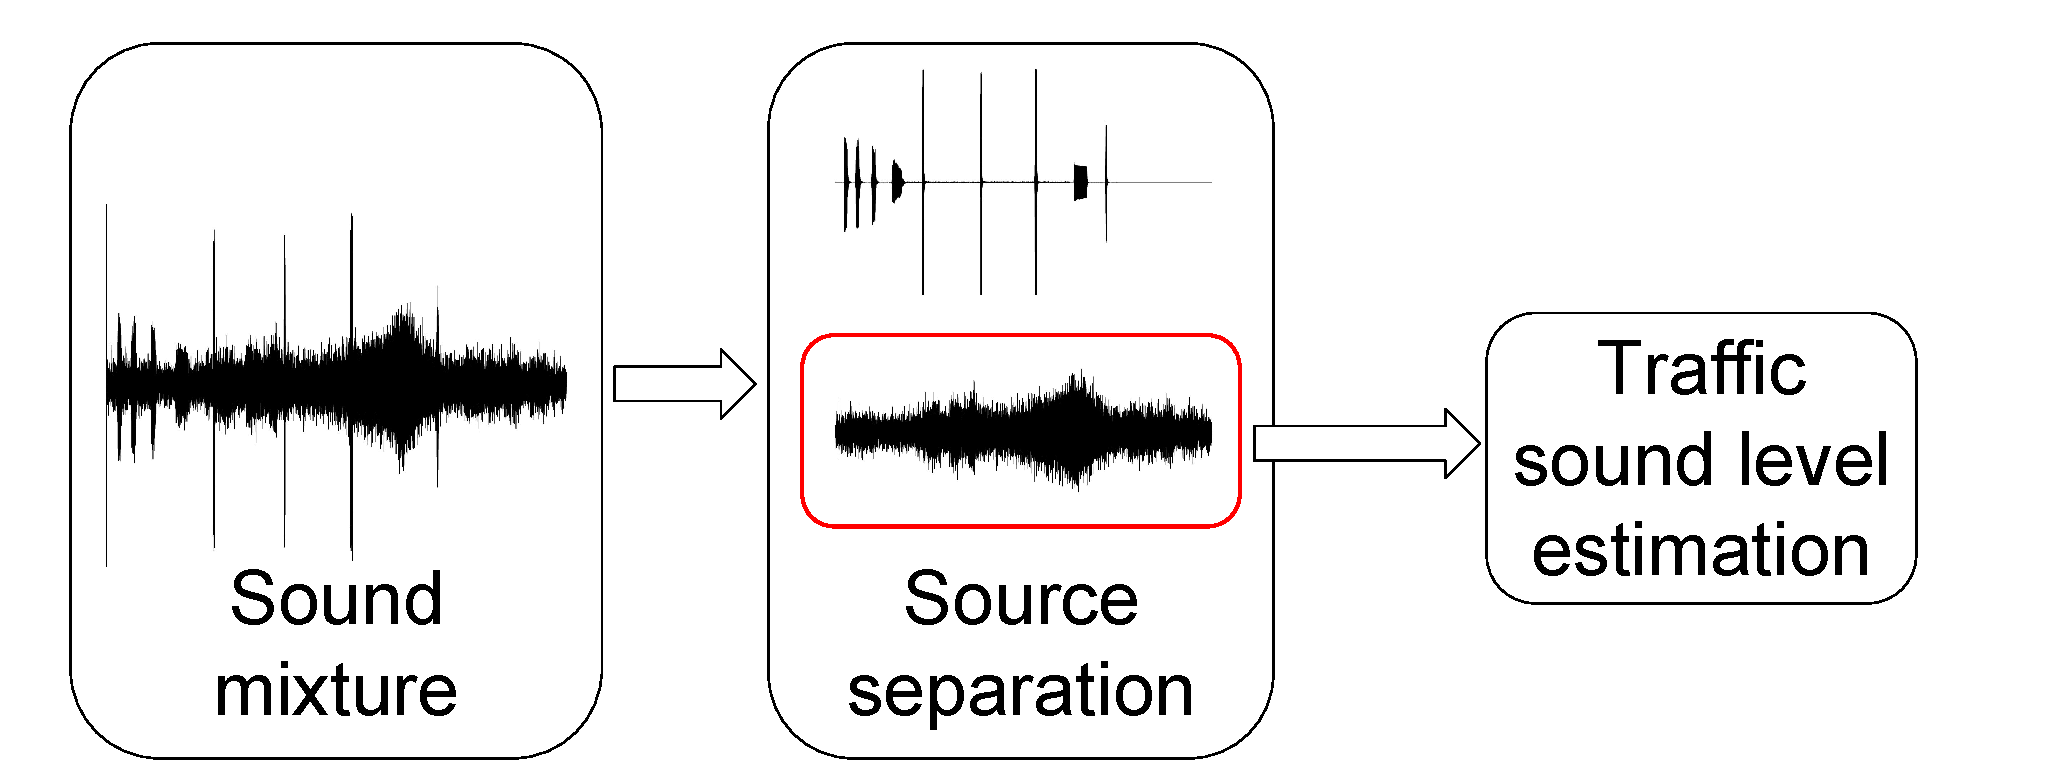
\includegraphics[width=.9\linewidth]{figures/bloc_diagram_source_separation.pdf}
\caption{Block diagram of the blind source separation model}
\label{fig:source_separation}
\end{figure}

All these measurement protocols allow the combination of measures and predictions to improve the accuracy of the produced noise maps. Traffic noise maps and measurements were compared on restrictive areas in \cite{lefebvre2017traffic} and \cite{mioduszewski2011noise}. Wei et al. \cite{wei_dynamic_2016} modify the acoustical parameters of the simulation thanks to noise measurements, while  Mallet et al. \cite{ventura2017estimation} call for data assimilation techniques between models and measurements to reduce the uncertainty of the produced noise maps. However, these works make the implicit assumption that the noise measurements consist mainly of road traffic. In the aim to improve road traffic noise maps, the use of measurements has first to deal with the challenge to estimate correctly the road traffic sound level.
Even if road traffic is predominant on many urban areas, urban sound environments are composed of many different overlapping sound sources (passing cars, voices, footsteps, car horn, whistling birds \dots), what makes the task of estimating correctly the traffic sound level within an urban sound mixture not trivial.

Many works have dealt with the classification \cite{valero2012hierarchical,shen_environmental_2012}, the detection \cite{luitel2016sound,mesaros2015sound} or the recognition \cite{defreville_automatic_2006,parascandolo_recurrent_2016} of urban sound events. In these cases, a two-step scheme is followed where audio samples are described with a set of features (Mel Frequency Cepstral Coefficient, MPEG-7 descriptors \dots) and classified with the help of a classifier (Gaussian Mixtures Models, Artificial Neural Network \dots) \cite{chu2008environmental, cowling_comparison_2003}. The classifier is learnt from a learning database and is next applied on a test database to validate the algorithms.
Dedicated to the traffic, in \cite{socoro_anomalous_2017}, an Anomalous Event Detection, based on MFCC features, is proposed with the specific aim to improve the traffic sound estimation. It is based on the detection of unwanted sound events in order to discard them.


An other approach, followed in this paper, is to consider the blind source separation paradigm which consists in the extraction of a specific signal inside a set of mixed signals, see Figure \ref{fig:source_separation}. From the different existing methods, Non-negative Matrix Factorization (NMF) \cite{lee_learning_1999}, appears to be a relevant method for monophonic sensor networks. Many applications can be found for musical \cite{smaragdis_non-negative_2003, benetos2006musical} and speech \cite{wilson_speech_2008, mysore2011non} contents. Dedicated to sound separation with environmental sounds, Immani and Kasa\"i \cite{satoshi_innami_nmf-based_2012} used NMF in a two steps sound separation with the help of time variant gain features. Dedicated to the traffic sound separation, a first study \cite{gloaguen2018Estimation} has been conducted, in which diverse NMF estimation rules are compared, namely the supervised, the semi-supervised, and the threshold initialized NMF, have been applied on a large set of simulated sound scenes. This corpus mixes 6 sound categories (\textit{alert, animals, climate, humans, mechanics, transportation}) with a traffic component calibrated to different sound levels, according to the other sound classes (in the rest of the document, these sound classes, not related to the traffic component, are resumed as the \textit{interfering} sound class), to obtain variable traffic predominance. 
The diversity of this corpus was made to assess the performances and the limits of each NMF formula. 
However, if this study reveals the interest of NMF for urban sound environments, the assessment of its performance on a corpus of realistic sound scenes must be carried out in order to implement it on a sensor network. 
Design urban sound mixtures makes it possible to access to many acoustic properties as the onset and offset time and the sound level of each sound class and especially the traffic component. The realistic aspect of such a corpus is essential to obtain sound scenes similar to recordings and to validate NMF performances. However, like all simulated process, the realism of the scenes must be perceptually verified. 

In this paper, an urban sound corpus based on annotated urban recordings, and whose degree of realism is assessed through a perceptual test, is designed in order to estimate the traffic sound level with the help of the NMF framework.
The different NMF approaches are described in section \ref{part:nmf}. Next, the corpus of urban sound scenes is presented in section \ref{part:urban_scene}, from the sound database built-up to its validation. The experimental protocol and the results are then presented and discussed in section \ref{part:expProtocol} and \ref{part:results}.

\section{Non-negative Matrix Factorization}\label{part:nmf}

Non-negative Matrix Factorization (NMF) is a linear approximation method proposed by Paatero and Tapper \cite{paatero1994positive} and popularized by Lee and Seung \cite{lee_learning_1999}. It consists in approximating a non negative matrix $\mathbf{V}$ $\in \mathbf{R}^+_{F \times N}$ by the product of two non negative matrices: $\mathbf{W}$, called \textit{dictionary} (or basis), and $\mathbf{H}$, called the \textit{matrix activation} with dimensions $F \times K$ and $K \times N$ respectively, 

\begin{equation}\label{eq:nmf}
\mathbf{V} \approx \mathbf{WH}.
\end{equation}

The choice of the dimensions is often made such as $F\times K + K \times N < F \times N$ so that NMF can be a low rank approximation. This condition however is not mandatory. When  applying NMF to audio data, $\mathbf{V}$ is usually considered as the magnitude spectrogram obtained by a Short-Time Fourier Transform, $\mathbf{W}$ includes audio spectra and $\mathbf{H}$ is equivalent to the temporal activation of each spectrum, see Figure \ref{fig:exampleNMF}. Because of the non-negativity constraint, only additive combinations between the elements of $\mathbf{W}$ are considered. 

\begin{figure}[t]
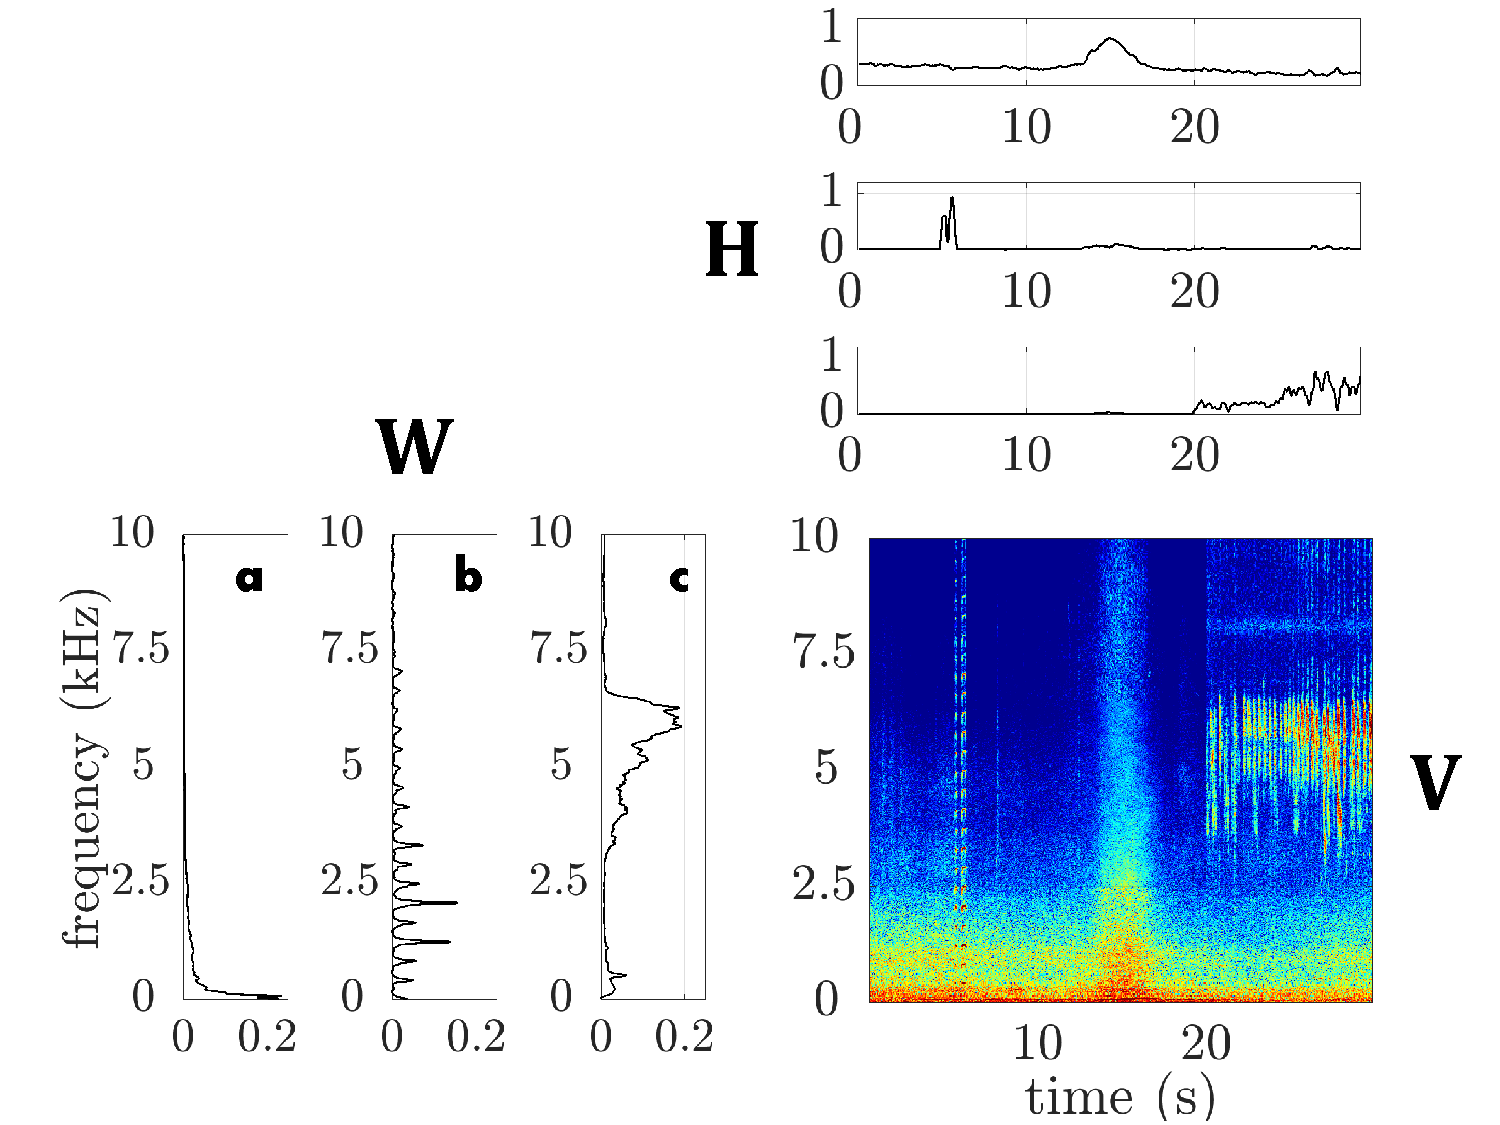
\includegraphics[width=.9\linewidth]{./figures/schema_introduction_nmf.pdf}
\caption{NMF decomposition of an audio spectrogram $V$ composed of 3 elements ($K$ = 3): passing car (a), car horn (b) and whistling bird (c).}
\label{fig:exampleNMF}
\end{figure}

The approximation of $\mathbf{V}$ by $\mathbf{WH}$ product is defined by a cost function to minimize,

\begin{equation}\label{eq:min-D-WH}
\underset{\mathbf{H} \geq 0, \mathbf{W} \geq 0}{\min} D\left(\mathbf{V} \Vert \mathbf{WH}\right),
\end{equation}

where $D(\bullet \Vert \bullet)$ is a divergence calculation such as:
\begin{equation}
D\left(\textbf{V} \vert\vert \mathbf{WH} \right) = \sum_{f = 1}^{F} \sum_{n = 1}^{N} d_{\beta}
\left(\textbf{V}_{fn} \vert \left[ \textbf{WH} \right]_{fn} \right).
\end{equation}

$d_{\beta}(x\vert y)$ is usually chosen as a $\beta$-divergence \cite{fevotte_algorithms_2011}, a sub-classes belonging to the Bregman divergences \cite{hennequin_beta-divergence_2011} which include 3 specific divergence calculations: the Euclidean distance (eq. \ref{eq:def_distEUC}), the Kullback-Leibler divergence (eq. \ref{eq:def_divKL}) and the Itakura-Sa\"{i}to divergence (eq. \ref{eq:def_divIS}):

\begin{subequations}\label{eq:divBetaGenerale}
\begin{numcases}{d_{\beta}(x\vert y) =}
    \frac{1}{2}(x-y)^2, & $\beta = 2$, \label{eq:def_distEUC}\\
    x\log \dfrac{x}{y} - x + y, & $\beta = 1$, \label{eq:def_divKL} \\
    \frac{x}{y} - \log \frac{x}{y} - 1 & $\beta = 0$. \label{eq:def_divIS}
\end{numcases}
\end{subequations}

The minimization problem (\ref{eq:min-D-WH}) is solved iteratively by updating the form of matrices $\mathbf{W}$ and $\mathbf{H}$. Different algorithms such as Alternating Least Square Method \cite{cichocki_regularized_2007} or Projected Gradient \cite{lin_projected_2007} have been considered. The most commonly used algorithm is the Multiplicative Update \cite{lee_algorithms_2000}. The latter method is chosen here, as it ensures non-negative results and the convergence of the results \cite{fevotte_algorithms_2011}.

\subsection{Supervised NMF}
The most easiest case of NMF is the one where the sound sources can be known \textit{a priori} and $\mathbf{W}$ can be built directly from audio samples. It leads to \textit{supervised} NMF (SUP-NMF). $\mathbf{H}$ is then the only matrix to estimate and is updated at every iteration (eq. \ref{eq:updateH}) \cite{fevotte_algorithms_2011}: 

\begin{equation} \label{eq:updateH}
\textbf{H}^{(i+1)} \leftarrow \textbf{H}^{(i)}\otimes\left(\frac{\textbf{W}^T \left[\left(\textbf{WH}^{(i)} \right)^{(\beta-2)}\otimes\textbf{V} \right]}{\textbf{W}^T \left[\textbf{WH}^{(i)} \right]^{(\beta-1)}}\right)^{\gamma(\beta)}
\end{equation}

with $\gamma(\beta) = \frac{1}{2-\beta},$ for $\beta < 1$, $ \gamma(\beta) = 1$, for $\beta \in \left[1,2\right]$ and $\gamma(\beta) = \frac{1}{\beta-1}$ for $\beta > 2$. Thus, the choice of the $\beta$-divergence in the equation \ref{eq:divBetaGenerale} affects how the matrix $\mathbf{H}$ is updated. The $A\otimes B$ and $A/B$ operators represent the Hadamard product and ratio.

Here, in an urban context, if the sound sources are known, their audio samples can be obtained to learn $\mathbf{W}$, see section \ref{part:dictionary_building}. As the position of each element is indexed, the traffic source separation from the other sound sources is made by extracting, from the dictionary and the activation matrix, the related elements:

\begin{equation}\label{eq:separationExtraction}
\mathbf{\tilde{V}}_{traffic} = \left[ \mathbf{WH} \right]_{traffic}.
\end{equation}

\subsection{Semi-supervised NMF}

The main issue with the supervised approach is the representational limit imposed by a fixed $\mathbf{W}$. To be completely successful, all the acoustical sources must be considered in the basis $\mathbf{W}$ which is not always possible in a complex urban environment. To overcome this issue, semi-supervised NMF (SEM-NMF) \cite{lee_semi-supervised_2010} has been proposed. It consists in decomposing, $\mathbf{W}_{F \times (K+J)}$ into two distinctive matrices: $\mathbf{W} = \left[ \mathbf{W_s}~\mathbf{W_r} \right]$ where $\mathbf{W_s}_{F \times K}$ is a fixed part of $\mathbf{W}$ composed of known audio spectra and $ \mathbf{W_r}_{F \times J}$, a mobile part which is updated, see eq. \ref{eq:W_r_SS}. Thus it is possible to let the method define the best elements to include in $\mathbf{W_r}$. Its dimension is set up as $J << K$ in order to consider, as a priority, the sound sources present in $\mathbf{W_s}$. $\mathbf{H}$ is then also decomposed in two matrices, $\mathbf{H}_{(K+J) \times N} = \genfrac[]{0pt}{0}{\mathbf{H_s}}{\mathbf{H_r}}$. Eq. \ref{eq:nmf} becomes

\begin{equation}
\mathbf{V} \approx \mathbf{WH} = \mathbf{W_s H_s}+\mathbf{W_r H_r}.
\end{equation}

$\mathbf{H_r}$ and $\mathbf{H_s}$ are updated separately, see eq. \ref{eq:H_r_SS} to eq. \ref{eq:H_s_SS}.


{\scriptsize
\begin{subequations}\label{eq:WH-SSupdate}
\begin{align}
\mathbf{W_r}^{(i+1)} &\leftarrow \mathbf{W_r}^{(i)}\otimes\left(\frac{\left[\left(\mathbf{W_r H_r}^{(i)} \right)^{(\beta-2)}\otimes\mathbf{V} \right]\mathbf{H_r}^T}{\left(\mathbf{W_r H_r}^{(i)} \right)^{(\beta-1)}\mathbf{H_r}^T}\right)^{\gamma(\beta)}, \label{eq:W_r_SS}\\
\mathbf{H_r}^{(i+1)} &\leftarrow \mathbf{H_r}^{(i)}\otimes\left(\frac{\mathbf{W_r}^T \left[\left(\mathbf{W_r H_r}^{(i)} \right)^{(\beta-2)}\otimes\mathbf{V} \right]}{\mathbf{W_r}^T \left(\mathbf{W_r H_r}^{(i)} \right)^{(\beta-1)}}\right)^{\gamma(\beta)},\label{eq:H_r_SS}\\
\mathbf{H_s}^{(i+1)} &\leftarrow \mathbf{H_s}^{(i)}\otimes\left(\frac{\mathbf{W_s}^T \left[\left(\mathbf{W_s H_s}^{(i)} \right)^{(\beta-2)}\otimes\mathbf{V} \right]}{\mathbf{W_s}^T \left(\mathbf{W_s H_s}^{(i)} \right)^{(\beta-1)}}\right)^{\gamma(\beta)}.\label{eq:H_s_SS}
\end{align}
\end{subequations}}

In this study, $\mathbf{W_s}$ is composed of traffic audio spectra, as it is the sound source of interest. Sources included in $\mathbf{W_r}$ are other sound sources (corresponding to the interfering class) that can be present in the urban sound scenes. The traffic signal estimation is next defined by the fixed part,

\begin{equation}\label{eq:separationExtraction_SS}
\mathbf{\tilde{V}}_{traffic} = \left[ \mathbf{W_s H_s} \right].
\end{equation}

The addition of $\mathbf{W_r}$ gives more flexibility to the method to represent correctly the spectrogram $\mathbf{V}$. The representational capability is increased, thus the approach is more adaptive to the different urban sound environments. Applications of SEM-NMF can be found for musical \cite{weninger2012supervised, kitamura_music_2014} and speech contents \cite{joder2012real, mysore2011non}.

\subsection{Thresholded Initialized NMF}\label{part:NMF_TI}

To allow even more flexibility while still considering prior knowledge of the source of interest, we propose a third approach based on the unsupervised NMF framework: Threshold Initialized NMF (TI-NMF). Usually, in unsupervised NMF, the dictionary is initiated randomly when there is no \textit{prior} knowledge on the sound sources present. Here, as the target sound source is known and the spectra are available, an initial dictionary, $\mathbf{W_0}$, is designed and then updated alternatively with $\mathbf{H}$,

\begin{equation}\label{eq:updateW_unsup}
\textbf{W}^{(i+1)} \leftarrow \mathbf{W}^{(i)}\otimes \left(\frac{\left[\left(\mathbf{W}^{(i)}\mathbf{H} \right)^{(\beta-2)}\otimes \mathbf{V} \right]\mathbf{H}^T}{\left[\mathbf{W}^{(i)}\mathbf{H} \right]^{(\beta-1)}\mathbf{H}^T}\right)^{\gamma(\beta)}.
\end{equation}

With this operation, $\mathbf{W_0}$ is oriented to the focused sound source (the road traffic) but also can be adapted to the content of the scene thanks to the updates. After $N$ iterations, each element $k$ of the final dictionary, $\mathbf{W'}$, is compared with its initial value in $\mathbf{W_0}$, in order to identify which element is stayed close to the traffic component. A cosine similarity $D_{\theta}\left(\mathbf{W_0} \Vert \mathbf{W'} \right)$ is computed for each element $k$ as it is scale-invariant and bounded,

\begin{equation}
D_{\theta}\left(\mathbf{w_0} \Vert \mathbf{w'} \right) = \frac{\mathbf{w_0}.\mathbf{w'}}{\Vert \mathbf{w_0}  \Vert . \Vert \mathbf{w'} \Vert}.
\end{equation}

where $\mathbf{w}$ is a $k$ element of $\mathbf{W}$ of $F \times 1$ dimensions. When $D_{\theta}\left(\mathbf{w_0} \Vert \mathbf{w'} \right)$=1, the element $\mathbf{w'}$ is identical to $\mathbf{w_0}$. If $D_{\theta}\left(\mathbf{w_0} \Vert \mathbf{w'} \right)$=1, both elements are fully different. The extraction of traffic elements in $\mathbf{W'}$ is carried out by a hard thresholding method \cite{donoho1994threshold}. It consists in weighting in a binary way $\mathbf{W'}$ according to $D_{\theta}\left(\mathbf{w_0} \Vert \mathbf{w'} \right)$ and a threshold value $\alpha_k$ such as:

%\ml{on pourrait tout a fait imaginer l'ajout d'élément de dictionaire random pour se rapprocher de la semi.}

\begin{equation}
\mathbf{w}_{traffic} = \alpha_k \mathbf{w'}.
\end{equation}
with
\begin{subequations}\label{eq:WH-TIupdateHard}
\begin{numcases}{\alpha_k =}
1  & iff \quad $D_{\theta}\left(\mathbf{w}_{0} \Vert \mathbf{w'} \right) > t_h$, \\
 0 & else.
\end{numcases}\\
\end{subequations}

To summarize, to approximate the audio spectrogram $\mathbf{V}$ and estimate the traffic component, 3 methods are used which deal differently with the \textit{a priori} knowledge on the traffic. SUP-NMF is only based on fixed \textit{traffic} elements and is constrained to used it to obtain $\mathbf{\tilde{V}}_{traffic}$. SEM-NMF completes this dictionary by the add of a mobile dictionary to better consider the interfering sound events and then offer more flexibility. Finally, TI-NMF considers first a dictionary composed of \textit{traffic} spectra, as SUP-NMF, but allows an update of them. The interest of an initiated dictionary is then to focus on the source of interest during the updates. This method therefore makes it more suitable for solving the generalization issues as it is the entire dictionary that can be fully adapted to the sound scenes. The elements that deviates too much from the originals spectra are then discarded by the thresholding step.

These above described methods are applied on an evaluation corpus, composed of simulated sound scenes, in order to compare the estimated traffic sound levels with an exact reference. This new sound corpus is designed by considering realistic urban sound environments with many kinds of mixed sound sources.

\section{Design of realistic urban sound scenes}\label{part:urban_scene}

\begin{figure*}[t]
\centering
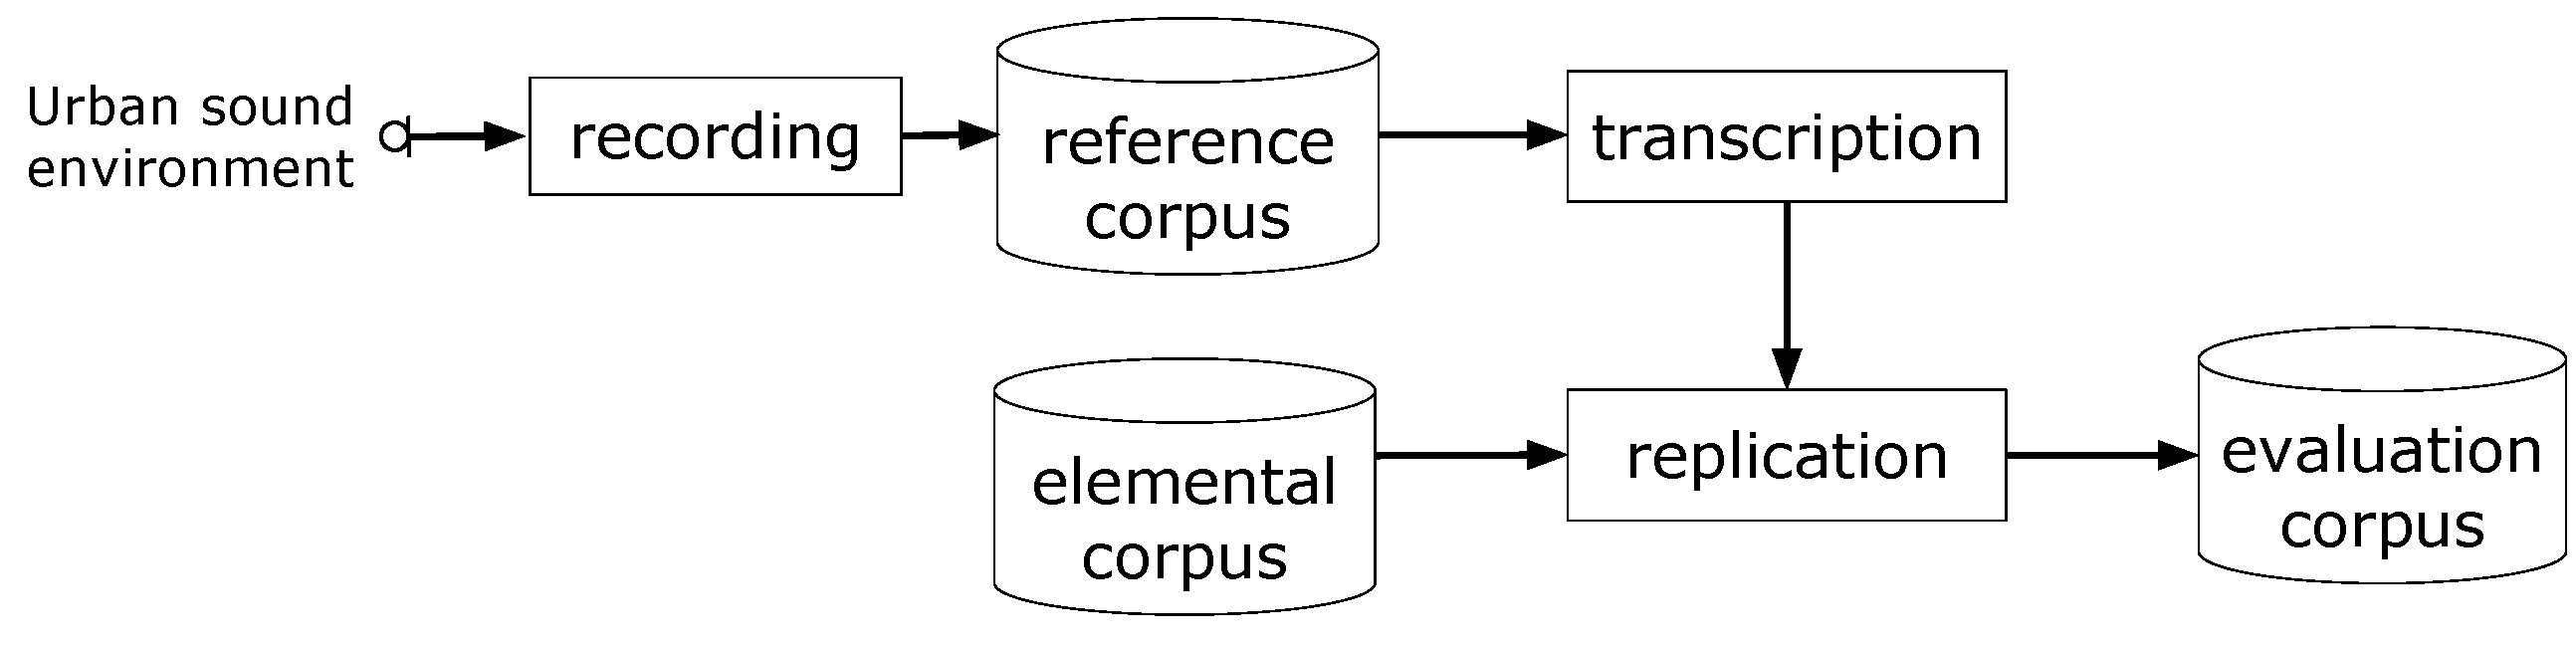
\includegraphics[width=0.8\linewidth]{./figures/realistic_urban_sound_scene_design.pdf}
\caption{Bloc diagram of the design of the evaluation corpus}
\label{fig:transcription}
\end{figure*}

The evaluation corpus must be both realistic and non ambiguous in terms of traffic sound level. The former calls for the use of real urban sound environments, and the latter imposes the use of controlled sound sources with known properties: onset and offset time location, and sound level. Indeed, the precise annotation of the sound level of a given source of interest in a real recording is a very complex problem. Two corpora are proposed to design a valid corpus of  evaluation. The first, called the reference corpus, is a set of recordings of urban sound environments, from which, what we call, a transcription is made, \textit{i.e.} which sound source is present from this time to this time. The second, called the elemental corpus, is a set of monophonic recordings of isolated sound sources that represent categories of events that are present in the reference scenes. The elemental corpus is built with still existing sounds and with specific recordings, see part \ref{part:simScene}. The evaluation corpus is then designed by replicating the reference corpus according to the transcription with the help of the elemental corpus, see Figure \ref{fig:transcription}.

The reference corpus is composed of 76 recordings from 2 to 5 min, achieved in the \nth{13} district of Paris (France) at 19 different locations \footnote{Recordings were made as part of the Grafic project funded by Ademe}, see Figure \ref{fig:map_grafic}, which cover various sound environments. A complete description of the experimental protocol can be found in \cite{aumond_modelling_2017}. Two of the 76 recordings are rejected for the analysis because the audio files were corrupted, resulting in 74 valid audio files assumed as representative of the variety of urban sound environments. The recordings are listened and categorized within four different sound environments, as proposed in \cite{can_describing_2015}: \textit{park} (8 audio files with a cumulative duration of 16min01), \textit{quiet street} (35 audio files with a cumulative duration of 77min27), \textit{noisy street} (23 audio files with a cumulative duration of 56min10) and \textit{very noisy street} (8 audio files with a cumulative duration of 21min42). Then, each audio file is transcripted, noticing the start, end time and level of each sound event along with its sound class. This annotation phase makes it possible to produce simulated sound scenes with the same positions of sound events than the recordings and therefore as close as possible to the real scenes.

\begin{figure}[t]
\centering
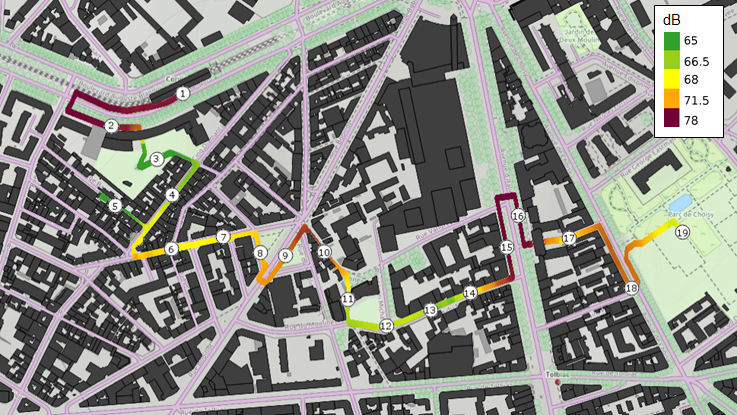
\includegraphics[width=\linewidth]{./figures/trajet_19pts.png}
\caption{Walked path with the 19 stop points  \cite{aumond_modelling_2017}.}
\label{fig:map_grafic}
\end{figure}


\subsection{Generation of the evaluation corpus}\label{part:simScene}
The sound scenes are generated with the \textit{SimScene} software\footnote{Open-source project available at: \url{https://bitbucket.org/mlagrange/simscene}}, \cite{rossignol_simscene:_2015}, a simulation software generating monaural sound mixtures in wav format from an isolated sounds database.
This software has already been used in a wide range of experiments for sound detection algorithm assessment \cite{lafay_new_2014, benetos2016detection}. The \textit{SimScene} software allows the design of several type of sequencing, from \textit{abstract} ones (time indexes and amplitudes are drawn from random distributions) to  precise ones, where the time indexes and amplitudes for each event are set by the user. The latter type is considered in this study. As output, \textit{SimScene} generates an audio file of the global sound mixture as well as for each sound class present in the scene, see Figure \ref{fig:example_simScene}. It makes it possible to know their exact contributions in the scene, in particular their sound levels.

\begin{figure}[t]
    \centering
       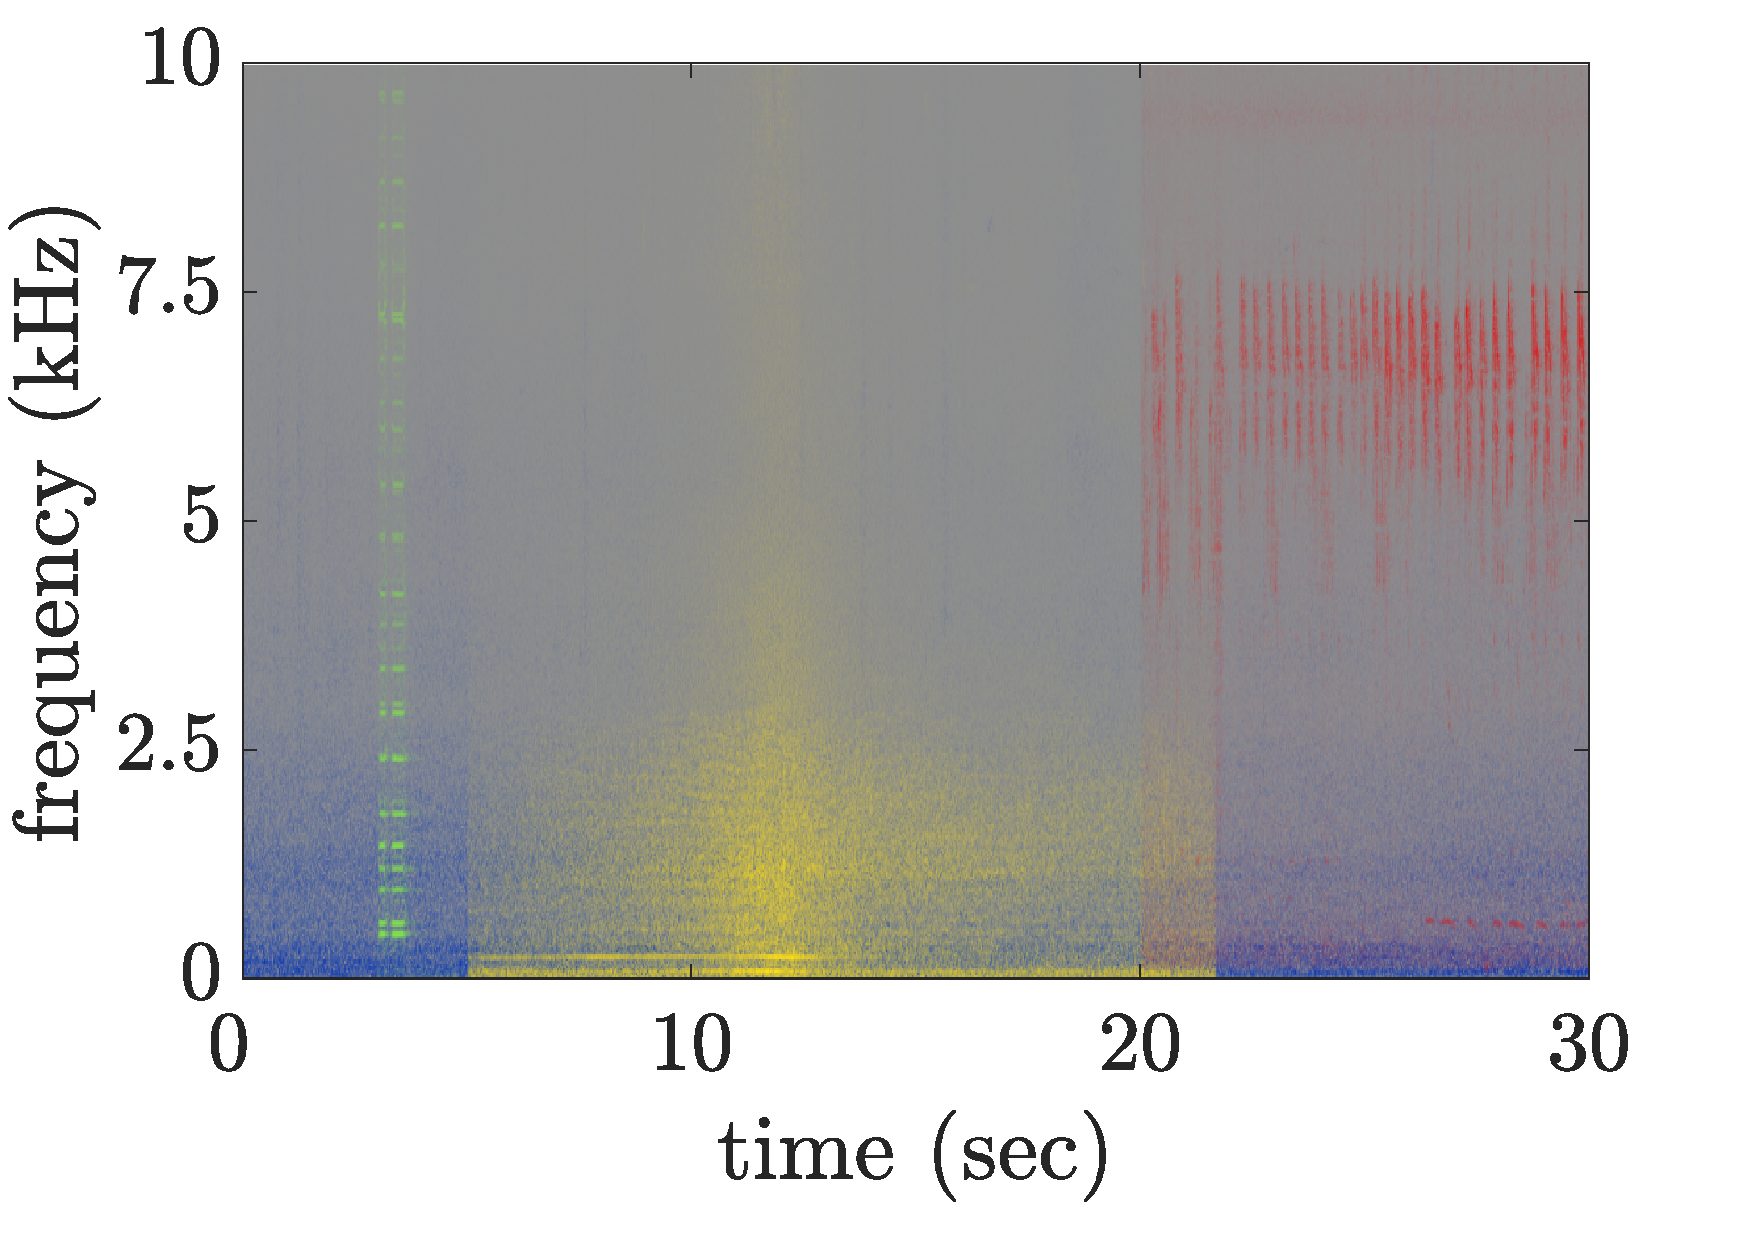
\includegraphics[width=.85\linewidth]{./figures/exampleSimScene.pdf}
    \caption{Spectrogram of a simple scene created with the \textit{SimScene} software with one sound background (road traffic in blue) and 3 sound events (car horn in green, passing car in yellow and whistling bird in red).}
    \label{fig:example_simScene}
\end{figure}

To replicate the 74 recordings in simulated scenes, a high quality (wav format, 44.1 kHz sampling rate, high \textit{Signal Noise Ratio}) elemental corpus has been built-up from audio samples found online (\textit{freesound.org}) or with the help of an already existing sound database \cite{salamon2014dataset}. The elemental corpus is composed of two categories of sound: the \textit{event} category, which includes 245 brief sound samples considered as salient, with a 1 to 20 seconds duration and classified among 21 sound classes (\textit{ringing bell, whistling bird, car horn, passing car, hammer, barking dog, siren, footstep, metallic noise, voice \dots}) and the \textit{background} (or \textit{texture}) category gathering 154 long duration sounds ($\approx$ 1mn30), whose acoustic properties do not vary in time. This category includes among others \textit{whistling bird, crowd noise, rain, children playing in schoolyard, constant traffic noise} sound classes. Each sound class is composed of multiple samples (\textit{carHorn01.wav, carHorn02.wav \dots}) that are randomly chosen by the \textit{simScene} software to bring diversity.
As the road traffic is the main component in urban environment and is the sound source of interest, recordings of car passages have been made on the Ifsttar's runway. The recordings have been made for 4 different cars (Renault Scenic, Renault M\'egane, Renault Clio and Dacia Sandero), at different speeds and gear ratios. Overall, 103 car passages have been recorded. In order to avoid overfitting issues, the audio samples of the first two cars (Renault Scenic and Renault M\'egane) are included in the \textit{SimScene}'s elemental corpus (50 audio files in total). The last 53 audio samples are dedicated to the dictionary design, $\mathbf{W}$ as part of NMF, see section \ref{part:dictionary_building}. A full description of the recordings can be found in \cite{gloaguen_creation_2017}.

\begin{table}[t]
\centering
\caption{Mean \textit{Traffic Interfering Ratio} and its standard deviation for each sound environment.}
\begin{tabular}{lc}
 & $mTIR$ (dB)\\ \hline
 \textit{park} & -9.10 ($\pm$ 7.35) \\
 \textit{quiet street} & 0.88 ($\pm$ 5.92) \\
 \textit{noisy street} & 6.96 ($\pm$ 5.16) \\
 \textit{very noisy street} & 15.75 ($\pm$ 9.78) \\ \hline
\end{tabular}
\label{tab:mTIR}
\end{table}

With this built-up corpus, the \textit{SimScene} software and the transcriptions of the recordings, 74 simulated sound scenes are generated, which have the same temporal structure of the reference recordings. The sound level of each sound class is adjusted manually on each sound scene to be faithful compared to the recorded scenes. To check this adjustment, the mean \textit{Traffic Interfering Ratio} ($mTIR$) is calculated, see Table \ref{tab:mTIR}. It expresses, on all the scenes of a sound environment, the mean difference between the equivalent traffic sound levels of each scene, $L_{p,traffic}$, with the sound level of the \textit{interfering} sound class, $L_{p, interfering}$, which gathered all the other sound sources not related to the traffic, see Eq. \ref{eq:mTIR}. It quantifies the predominance of the traffic component for the 4 types of sound environments, 

\begin{equation}\label{eq:mTIR}
mTIR = \frac{\sum_{i = 1}^M L_{p,traffic} - L_{p, interfering}}{M}.
\end{equation}

where $M$ is the number of available scenes for each sound environment ($M$ = 8 for \textit{park} environment, $M$ = 35 for \textit{quiet street} environment, $M$ = 23 for \textit{noisy street} environment and $M$ = 8 for \textit{very noisy street} environment). The $mTIR$ is always negative for the \textit{park} as it is the sound environment where the traffic is less present. The \textit{interfering} sound class is therefore the main sound source which is coherent with this kind of environment. The $mTIR$ can be positive or negative depending on the traffic presence on the scene in the case of the \textit{quiet street}. For the 2 others sound environments, when the traffic becomes the main sound source, $mTIR$ is always positive.

\subsection{Perceptual test}

To evaluate the level of realism of the evaluation corpus composed of replicated urban sound scenes, a perceptual test is considered.

The perceptual test is conducted with a panel of 50 listeners that are asked to assess the level of realism on a 7-point scale (1 is \textit{not realistic at all}, 7 is \textit{very realistic}) of a set of replicated and recorded scenes. The total number of sound scenes tested is set at 40. This is less than the number of scenes available to ensure that each audio sample is sufficiently assess. The first half includes 20 30-seconds audio files corresponding to the real scenes, including 5 scenes that belong to the sound environment \textit{park}, 6 from \textit{quiet street}, 4 from \textit{noisy street} and 5 from \textit{very noisy street} chosen randomly among the recorded scenes. The second half is composed of the replicated scenes from the evaluation corpus corresponding to the same 20 reference scenes. In order to limit the duration of the test to preserve the concentration of the subjects, each subject listens to only a subset of 20 sound scenes. All the scenes are normalized to the same sound level, chosen at 65 dB, and the subjects are not allowed to change the output sound level once set at the beginning of the experiment.

The experimental design is elaborated following a partially Balanced Incomplete Block Design (PBIBD) \cite{john1977optimal} the audio allocated to each participant and the listening order. This process allows to each sound sample to be assessed almost the same number of time and to avoid statistical biais. The experimental design and the listening order per participant are performed with the package \textit{sensoMineR} on the \textit{R} software \cite{le_sensominer:_2008}.\\

The test was available online from February 8th, 2017 and the needed number of participant (50) has been reached 12 days later. During the test, the participants had the possibility to listen to each scene as many times as wanted before assessing, without being able to change their judgment afterwards. The participants could also leave a comment on each audio to explain the rating \footnote{The interface of the experiment is available \url{http://soundthings.org/research/xpRealism}}. Based on the information provided, the panel of 50 listeners was made of 31 males and 18 females (one not documented) with an average age of 36 ($\pm$ 12) years old. $62\%$ of the participants declared having no experience in the listening of urban sound mixtures. 
The results show that the average score (with its standard deviation) of all the replicated scenes ($m_{replicated}$ = 5.1 ($\pm$ 1.6)) is close to the recorded ones ($m_{recorded}$ = 4.9 ($\pm$ 1.6)). To determine whether a replicated scene is perceived in a similar way to that recorded, a Student's t-test is performed, for each scene, between the scores from the recorded sample and those from the replicated sample with the $H_0$ hypothesis which considers the similarity between the distribution of the rates for the recorded and the replicated scenes of each participant with a \textit{p-value} threshold of 5$\%$.  The 20 performed t-tests show that the differences in the assessment of the replicated and the recorded scene, according to their degree or realism, is not significant (p-value$>5\%$).

More details on the results can be found in  \cite{gloaguen_creation_2017}. As the perceived realism of the replicated and the recorded scenes are not significantly different, we consider that  these sound mixtures are relevant to assess the performances of NMF according to the traffic sound level estimate.

\begin{figure*}[t]
\centering
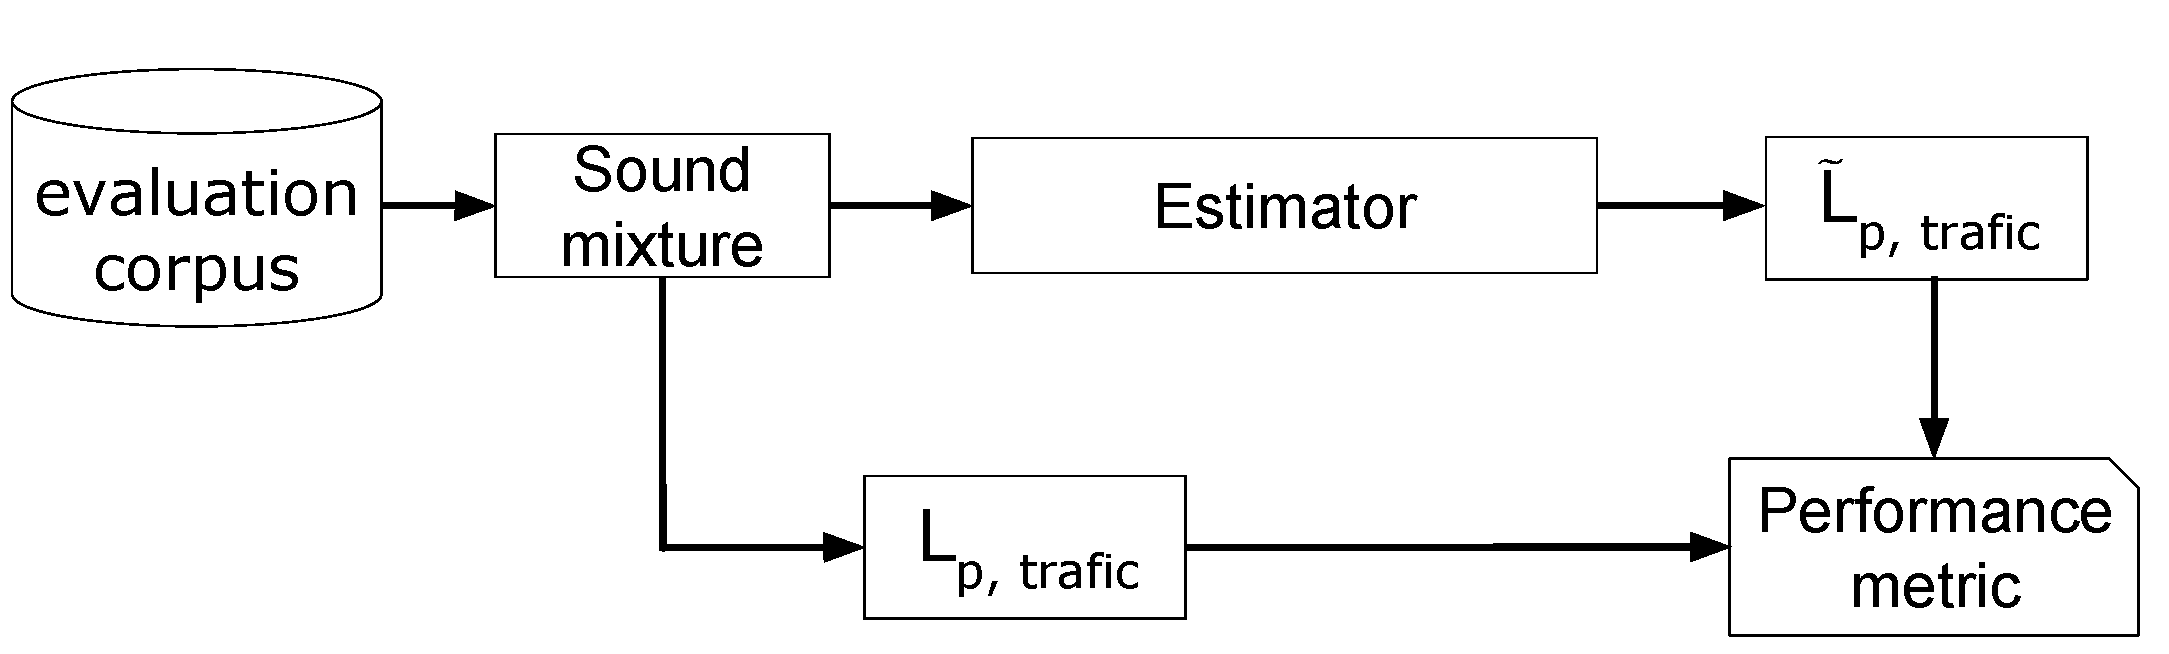
\includegraphics[width=0.7\linewidth]{figures/bloc_diagram_estimator.pdf}
\caption{Bloc diagram of the different stages for the estimation of the traffic sound level.}
\label{fig:bloc_diagram_estimator}
\end{figure*}

\section{Methods for the performance evaluation}\label{part:expProtocol}

The experiment aims at evaluating in a meaningful manner the performance of the NMF approach. To do so, the 74 replicated sound scenes, organized on 4 different types of sound environments are iteratively fed to the estimator which output an estimate of the equivalent sound level of the traffic within each scene $\tilde{L}_{p, traffic}$ (dB). This result is then compared to the reference sound level value given by the simulation process, $L_{p,traffic}$, see Figure \ref{fig:bloc_diagram_estimator}.



\begin{figure*}[t]
\centering
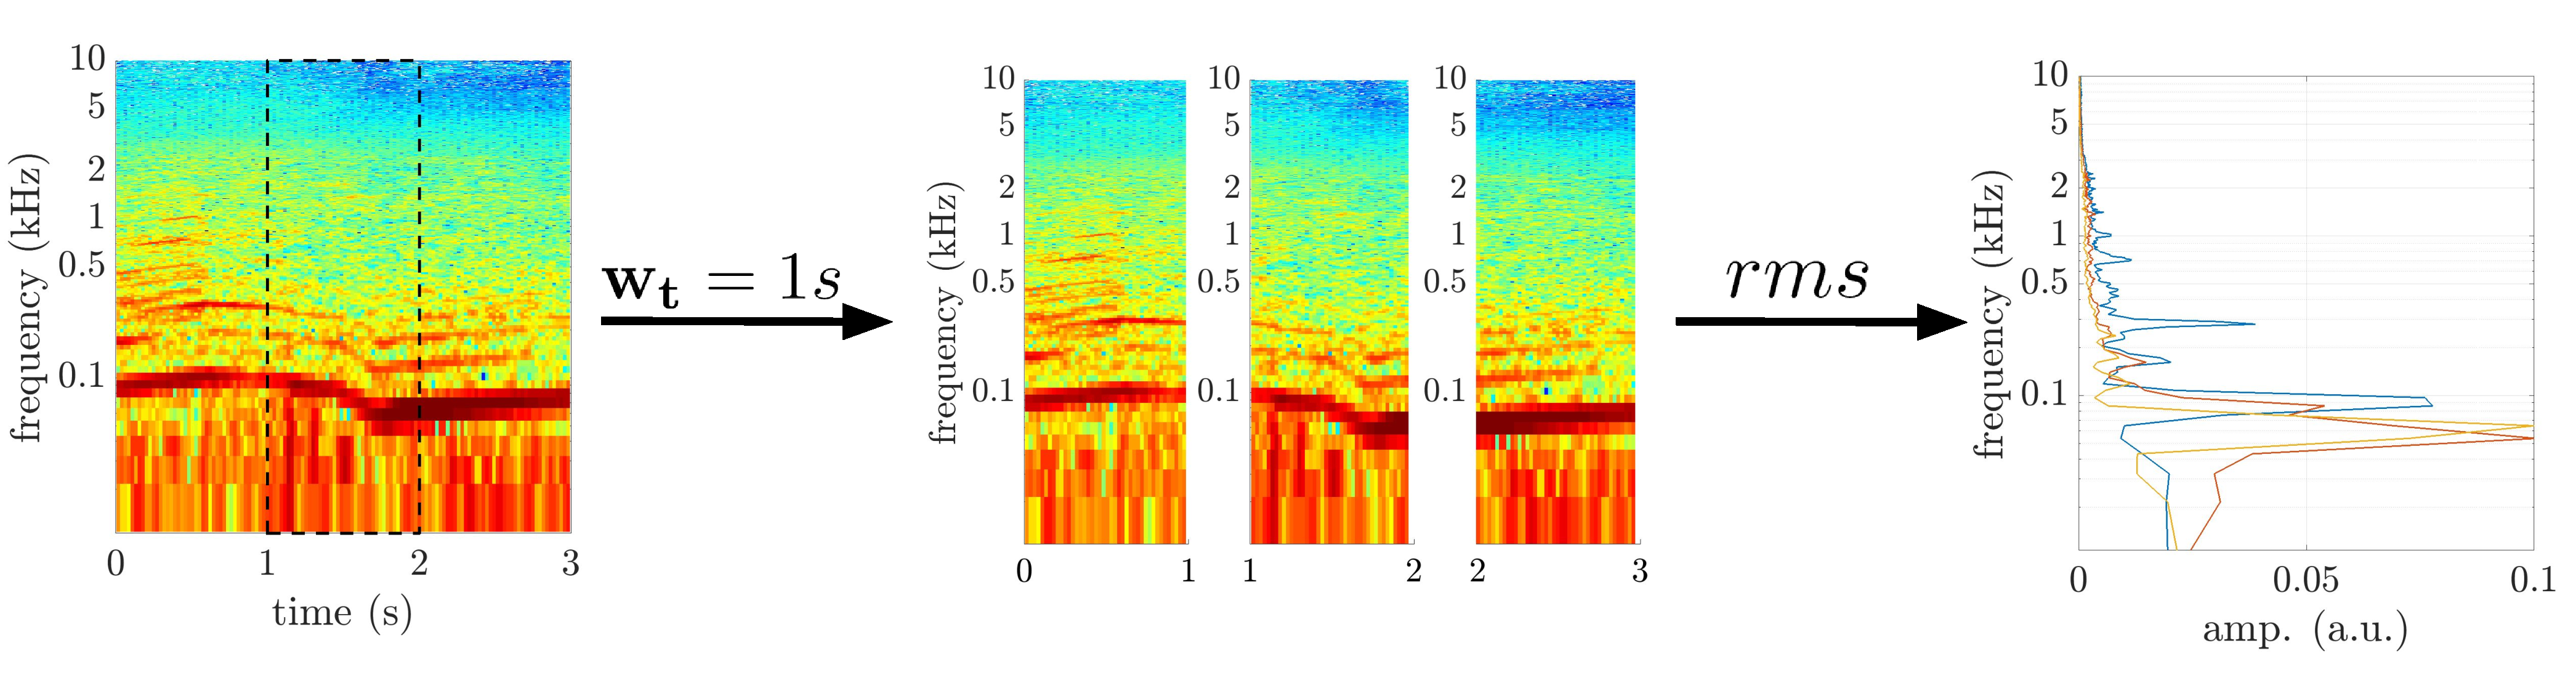
\includegraphics[width=\linewidth]{figures/extractionDictionary3.pdf}
\caption{Dictionary building on a 3 second example of a passing car with $\mathbf{w_t} = 1$ second, in dashed line a temporal frame of 1 s. In this case, the dictionary $\mathbf{W}$ is made of 3 spectra, each representative of a texture frame of $\mathbf{w_t}$ duration.}
\label{fig:example_dictionary}
\end{figure*}

\subsection{Reference estimator}

A reference estimator is necessary to be able to compare the performances of the different NMF-methods. As the road traffic is mainly composed of a low frequency content, a frequency low-pass filter (LP filter) is considered as baseline. The estimation of the traffic sound level with this reference estimator is simply the sound level after low-pass filtering, 

\begin{equation}
\mathbf{\tilde{V}}_{traffic} = \mathbf{V}_{f_c}.
\end{equation}

Different cut-off frequencies have been chosen such as $f_c \in \lbrace$500, 1k, 2k, 5k, 10k, 20k$\rbrace$ Hz. The experimental factors related to this estimator are summarized in Table \ref{tab:experimental_factorsFilter}.

The second estimator is based on the three NMF formula presented in part \ref{part:nmf} (see Figure \ref{fig:bloc_diagram_nmf}). Multiple experimental factors are involved in this second estimator where each of them having different modalities.

\begin{figure}[t]
\centering
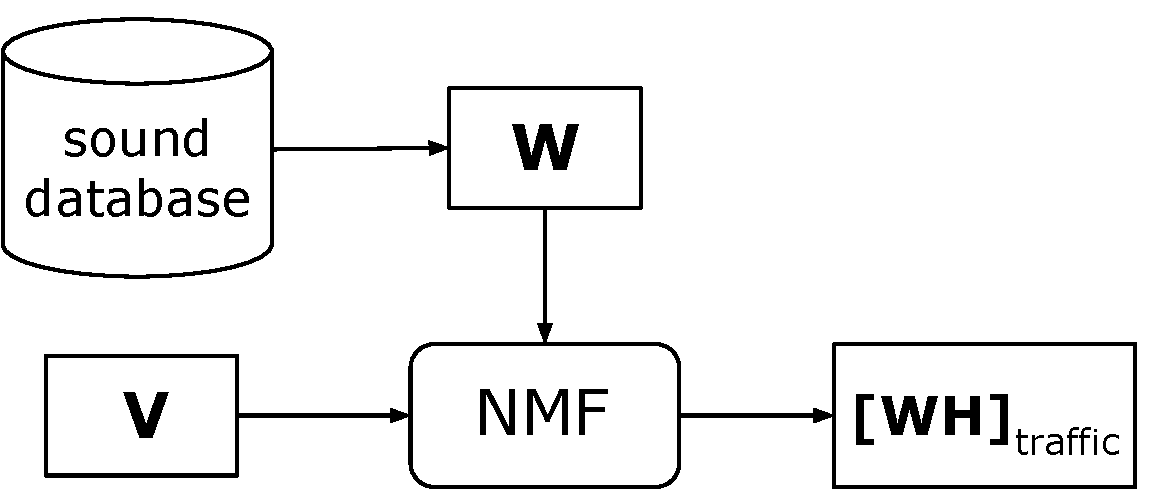
\includegraphics[width=.9\linewidth]{figures/bloc_diagram_NMF_EN_2.pdf}
\caption{Bloc diagram of the NMF estimator.}
\label{fig:bloc_diagram_nmf}
\end{figure}

\subsection{Dictionary building for NMF-methods}\label{part:dictionary_building}

The dictionary is designed from a sound database specially dedicated to this task. To prevent any overfitting issues, it contains the 53 audio files of the 2 cars not included  in the creation of the evaluation corpus, see part \ref{part:simScene}.

First the spectrogram of each audio file is computed ($w = 2^{12}$ sample points with 50 $\%$ overlap). The spectrogram is then cut in multiple temporal frames of $\mathbf{w_t}  \in \lbrace$0.5, 1$\rbrace$ second duration. In each frame, the root mean square on each frequency bin is calculated to obtained a spectrum of $F \times 1$ dimension. This method allows the description of the audio sample with a finer spectra and then having the different characteristic pitches of the traffic spectra. An illustrative example on a 3 seconds sample is displayed in Figure \ref{fig:example_dictionary}. From the 53 audio files, we obtain respectively 2218 elements for $\mathbf{w_t} = 0.5$ second and 1109 elements for $\mathbf{w_t} = 1$ second.

A $\mathbf{K}$-means clustering algorithm is applied to those elements to reduce these dimensions to $\mathbf{K} \in \lbrace$25, 50, 100, 200$\rbrace$ in order to avoid redundant information and decrease the computation time. The resulting $\mathbf{K}$ cluster centroids are taken as the elements of $\mathbf{W}$. Each basis of $\mathbf{W}$ is then normalized as $ \Vert \mathbf{w} \Vert = 1$ where $\Vert \bullet \Vert$ is the $\ell_1$ norm. Table \ref{tab:experimental_factorsNMF} summarizes the different modalities of the two experimental factors ($\mathbf{K}$ and $\mathbf{w_t}$).

\subsection{NMF experimental factors}

NMF is performed for 3 $\beta$-divergences: $\beta$ = 2 (Euclidean distance), $\beta$ = 1 (Kullback-Leibler divergence) and $\beta = 0$ (Itakura-Sa\"ito divergence). The spectrogram $\mathbf{V}$ and the dictionary $\mathbf{W}$ are expressed in a logarithmic scale through a third octave band representation that reduces the high frequency predominance where the traffic component is absent. In addition, as the number of frequency bins is reduced ($F$ = 29), the computation time is reduced too. 400 iterations are performed to get a stabilized results. For SEM-NMF, the number of elements in $\mathbf{W_r}$ is set to $J = 2$. For hard thresholding, the threshold value, $\mathbf{t_h}$ is set between 0.30 and 0.60 with a 0.01 increment.
Each unique association of modalities between each experimental factor forms an experimental setting. For the filter estimator, 24 settings are computed (4 $\times$ 6). For SUP and SEM-NMF, 192 settings are computed (4 $\times$ 2 $\times$ 2 $\times$ 4 $\times$ 3). Finally, for TI-NMF, the number of settings is much higher (2976) due to the higher cardinality of the set of threshold values (4 $\times$ 1 $\times$ 2 $\times$ 4  $\times$ 3 $\times$ 31).
The experimental factors and their different modalities are displayed in Tables \ref{tab:experimental_factorsFilter} and \ref{tab:experimental_factorsNMF}.

The approximated traffic spectrograms $\mathbf{\tilde{V}}_{traffic}$ are obtained after 400 iterations. The estimated traffic sound level in dB, $\tilde{L}_{p, traffic}$, is then computed,

\begin{equation}
\tilde{L}_{p, traffic} = 20\log\left(\frac{p_{rms}}{p_0}\right),
\end{equation}

where $p_0$ is the reference sound pressure, $p_0 = 2\times 10^{-5}$ Pa. For each setting, $M$ traffic sound levels, corresponding to the $M$ scenes of each sound environment, are then calculated.

\begin{table*}[t]
\caption{Experimental factors and their modalities for the frequency low-pass filter baseline estimator.}
\centering
\begin{tabularx}{17.5cm}{L{3cm}@{}C{12cm}@{}C{2cm}@{}}
	\hline
    \textbf{\begin{tabular}[c]{@{}l@{}}experimental \\ factors\end{tabular}} & \textbf{modalities} & \begin{tabular}[c]{@{}C{2cm}@{}}\textbf{number of}\\ \textbf{modalities}\end{tabular}\\ \toprule
\end{tabularx}

\begin{tabularx}{17.5cm}{L{3cm}@{}C{3cm}@{}@{}C{3cm}@{}@{}C{3cm}@{}@{}C{3cm}@{}C{2cm}@{}}
    \textbf{sound environment} & \begin{tabular}[c]{@{}c@{}}park\\ 'P'\end{tabular} & \begin{tabular}[c]{@{}c@{}}quiet street\\ 'Q'\end{tabular} & \begin{tabular}[c]{@{}c@{}}noisy street\\ 'N' \end{tabular}& \begin{tabular}[c]{@{}c@{}}very noisy street\\ 'vN'\end{tabular} & 4\\
\end{tabularx}

\begin{tabularx}{17.5cm}{L{3cm}@{}@{}C{2cm}@{}@{}C{2cm}@{}@{}C{2cm}@{}@{}C{2cm}@{}@{}C{2cm}@{}@{}C{2cm}@{}C{2cm}@{}}
\rowcolor[HTML]{C0C0C0}
   $\mathbf{f_c}$ (kHz) & 0.5 & 1 & 2 &  5 & 10 & 20 & 6\\
   \bottomrule
\end{tabularx}

\label{tab:experimental_factorsFilter}
\end{table*}


\begin{table*}[t]
\centering
\caption{Experimental factors and their modalities for the NMF estimator.}
\begin{tabularx}{17.5cm}{L{3cm}@{}C{12cm}@{}C{2cm}@{}}
	\hline
    \textbf{\begin{tabular}[c]{@{}l@{}}experimental \\ factors\end{tabular}} & \textbf{modalities} & \begin{tabular}[c]{@{}C{2cm}@{}}\textbf{number of}\\ \textbf{modalities}\end{tabular}\\ \toprule
\end{tabularx}

\begin{tabularx}{17.5cm}{L{3cm}@{}C{3cm}@{}@{}C{3cm}@{}@{}C{3cm}@{}@{}C{3cm}@{}C{2cm}@{}}
    \textbf{sound environment} & \begin{tabular}[c]{@{}c@{}}park\\ 'P'\end{tabular} & \begin{tabular}[c]{@{}c@{}}quiet street\\ 'Q'\end{tabular} & \begin{tabular}[c]{@{}c@{}}noisy street\\ 'N' \end{tabular}& \begin{tabular}[c]{@{}c@{}}very noisy street\\ 'vN'\end{tabular} & 4\\
\end{tabularx}

\begin{tabularx}{17.5cm}{L{3cm}@{}C{4cm}@{}@{}@{}C{4cm}@{}@{}C{4cm}@{}C{2cm}@{}}
	\rowcolor[HTML]{C0C0C0}
  \textbf{method} & SUP NMF & SEM NMF & TI NMF & 3\\
\end{tabularx}

\begin{tabularx}{17.5cm}{L{3cm}@{}C{6cm}@{}@{}C{6cm}@{}C{2cm}@{}}
    $\mathbf{w_t}$ (s)& 0.5 & 1 & 2 \\
\end{tabularx}

\begin{tabularx}{17.5cm}{L{3cm}@{}C{3cm}@{}@{}C{3cm}@{}@{}C{3cm}@{}@{}C{3cm}@{}C{2cm}@{}}
	\rowcolor[HTML]{C0C0C0}
    $\mathbf{K}$ & 25 & 50 & 100 & 200 & 4\\
\end{tabularx}


\begin{tabularx}{17.5cm}{L{3cm}@{}C{4cm}@{}@{}C{4cm}@{}@{}C{4cm}@{}C{2cm}@{}}
   $\mathbf{\beta}$ & 0 & 1 & 2 & 3\\
\end{tabularx}

\begin{tabularx}{17.5cm}{L{3cm}@{}C{12cm}@{}C{2cm}@{}}
	\rowcolor[HTML]{C0C0C0}
   hard threshold $\mathbf{t_h}$ & from 0.30 to 0.60 with a 0.01 step & 31\\
   \bottomrule
\end{tabularx}
\label{tab:experimental_factorsNMF}
\end{table*}

\subsection{Metrics}

The traffic sound levels, $\tilde{L}_{p,traffic}$, are compared to the exact values, $L_{p,traffic}$, through the Mean Absolute Error ($MAE$) \cite{willmott2005advantages}. The $MAE$ consists in the average across of the absolute difference between the exact and the estimated sound levels,

\begin{equation}
MAE_j = \left[\frac{\sum_{i = 1}^{M} \vert L_{p,traffic}^i - \tilde{L}_{p,traffic}^i \vert}{M}\right]_j,
\end{equation}

for each setting $j$. But it is also possible to average this metric according to the 4 different sound environments, through the mean $MAE$ error $mMAE$, to estimate the optimal setting that offers the lowest error for all the sound environments:

\begin{equation}
mMAE = \frac{\sum_{i = 1}^4 MAE_i}{4},
\end{equation}

where the other experimental factors (estimator, $f_c$, $\mathbf{K}$, $\mathbf{w_t}$, $\beta$, threshold value $\mathbf{t_h}$) are fixed.


\section{Results and discussion}\label{part:results}

Table \ref{tab:results} summarizes the lowest $mMAE$ errors according to the estimator (LP filter, NMF) and $\beta$ with the best setting of the experimental factors.

\begin{table*}[t]
\centering
\caption{Best $mMAE$ errors according to the experimental factor $\beta$ and the traffic sound level assessment method (in bold letter, the lowest error).}
\begin{tabular}{@{}ccccccc@{}}
\toprule
\textbf{method} & $f_c$ (kHz) & $\mathbf{\beta}$ & $\mathbf{K}$ & $\mathbf{w_t}$ (s) &  $\mathbf{t_h}$ &  \textbf{$mMAE$} (dB) \\ \midrule
filter & 20 & - & - & - & - & 3.76 ($\pm$ 4.35) \\
filter & 0.5 & - & - & - & - & 2.14 ($\pm$ 1.83) \\
\hline \hline
SUP-NMF & - & 0 & 200 & 0.5 & - & 4.06 ($\pm$ 4.69) \\
SUP-NMF & - & 1 & 200 & 0.5 & - & 2.79 ($\pm$ 3.38) \\
SUP-NMF & - & 2 & 25 & 1 & - & 2.32  ($\pm$ 2.80) \\
\hline \hline
SEM-NMF & - & 0 & 200 & 1 & - & 2.05 ($\pm$ 0.70) \\
SEM-NMF & - & 1 & 200 & 1 & - & 1.94 ($\pm$ 0.38) \\
SEM-NMF & - & 2 & 200 & 1 & - & 2.39 ($\pm$ 1.23) \\
\hline \hline
TI-NMF & - & 0 & 25 & 1 & 0.39 & 1.42 ($\pm$ 0.89)\\
TI-NMF & - & 1 & 100 & 1 & 0.35 & 1.38 ($\pm$ 0.88)\\
\textbf{TI-NMF }& - & \textbf{2} & \textbf{200} & \textbf{0.5} & \textbf{0.32} & \textbf{1.24 ($\pm$ 1.24)}\\
\bottomrule
\end{tabular}
\label{tab:results}
\end{table*}

The LP filter with $f_c = 20$ kHz cut-off frequency is equivalent to consider the sound level of the entire scene without specific distinction between the sound sources. The error is then important with a high standard deviation ($mMAE =$ 3.76 ($\pm$ 4.35) dB). The lowest error for a LP filter is obtained with $f_c$ = 500 Hz ($mMAE =$ 2.14 ($\pm$ 1.83) dB).

When considering all the sound scenes, SUP-NMF does not succeed to achieve a lower error than the 500 Hz LP filter for all the $\beta$ values. By adding the mobile part $\mathbf{W_r}$ in the dictionary, SEM-NMF with $\beta = 0$ and $\beta = 1$ allows a lower error than 500 Hz LP filter with a reduced standard deviation especially for $\beta = 1$ ($mMAE = 1.94$ ($\pm$ 0.38) dB).

TI-NMF is the approach with the lowest global error ($<$ 1.50 dB). The best result is obtained for TI-NMF ($MAE$ = 1.24 ($\pm$ 1.24) dB) with $\beta = 2$, $\mathbf{K}$ = 200, $\mathbf{w_t}$ = 0.5 s and as threshold value $\mathbf{t_h}$ = 0.32. This combination of settings offers the most efficient method adapted to the different sound environments.
Furthermore, on the dictionary creation, only SEM-NMF proposes the same dictionary design for all the best methods according to $\beta$. In the opposite, SUP and TI-NMF propose different associations between $\mathbf{K}$ and $\mathbf{w_t}$. One can notice that, through the 3 methods, it is mainly a high number of elements in $\mathbf{K}$ (100, 200) that is preferred. With more elements, it makes it possible to resolve easily the generalization issue. 

From these global results, the $MAE$ errors are compared to the LP filter and each method for the 4 types of sound environments, see Figure \ref{fig:mae_env}.

\begin{figure}[t]
\centering
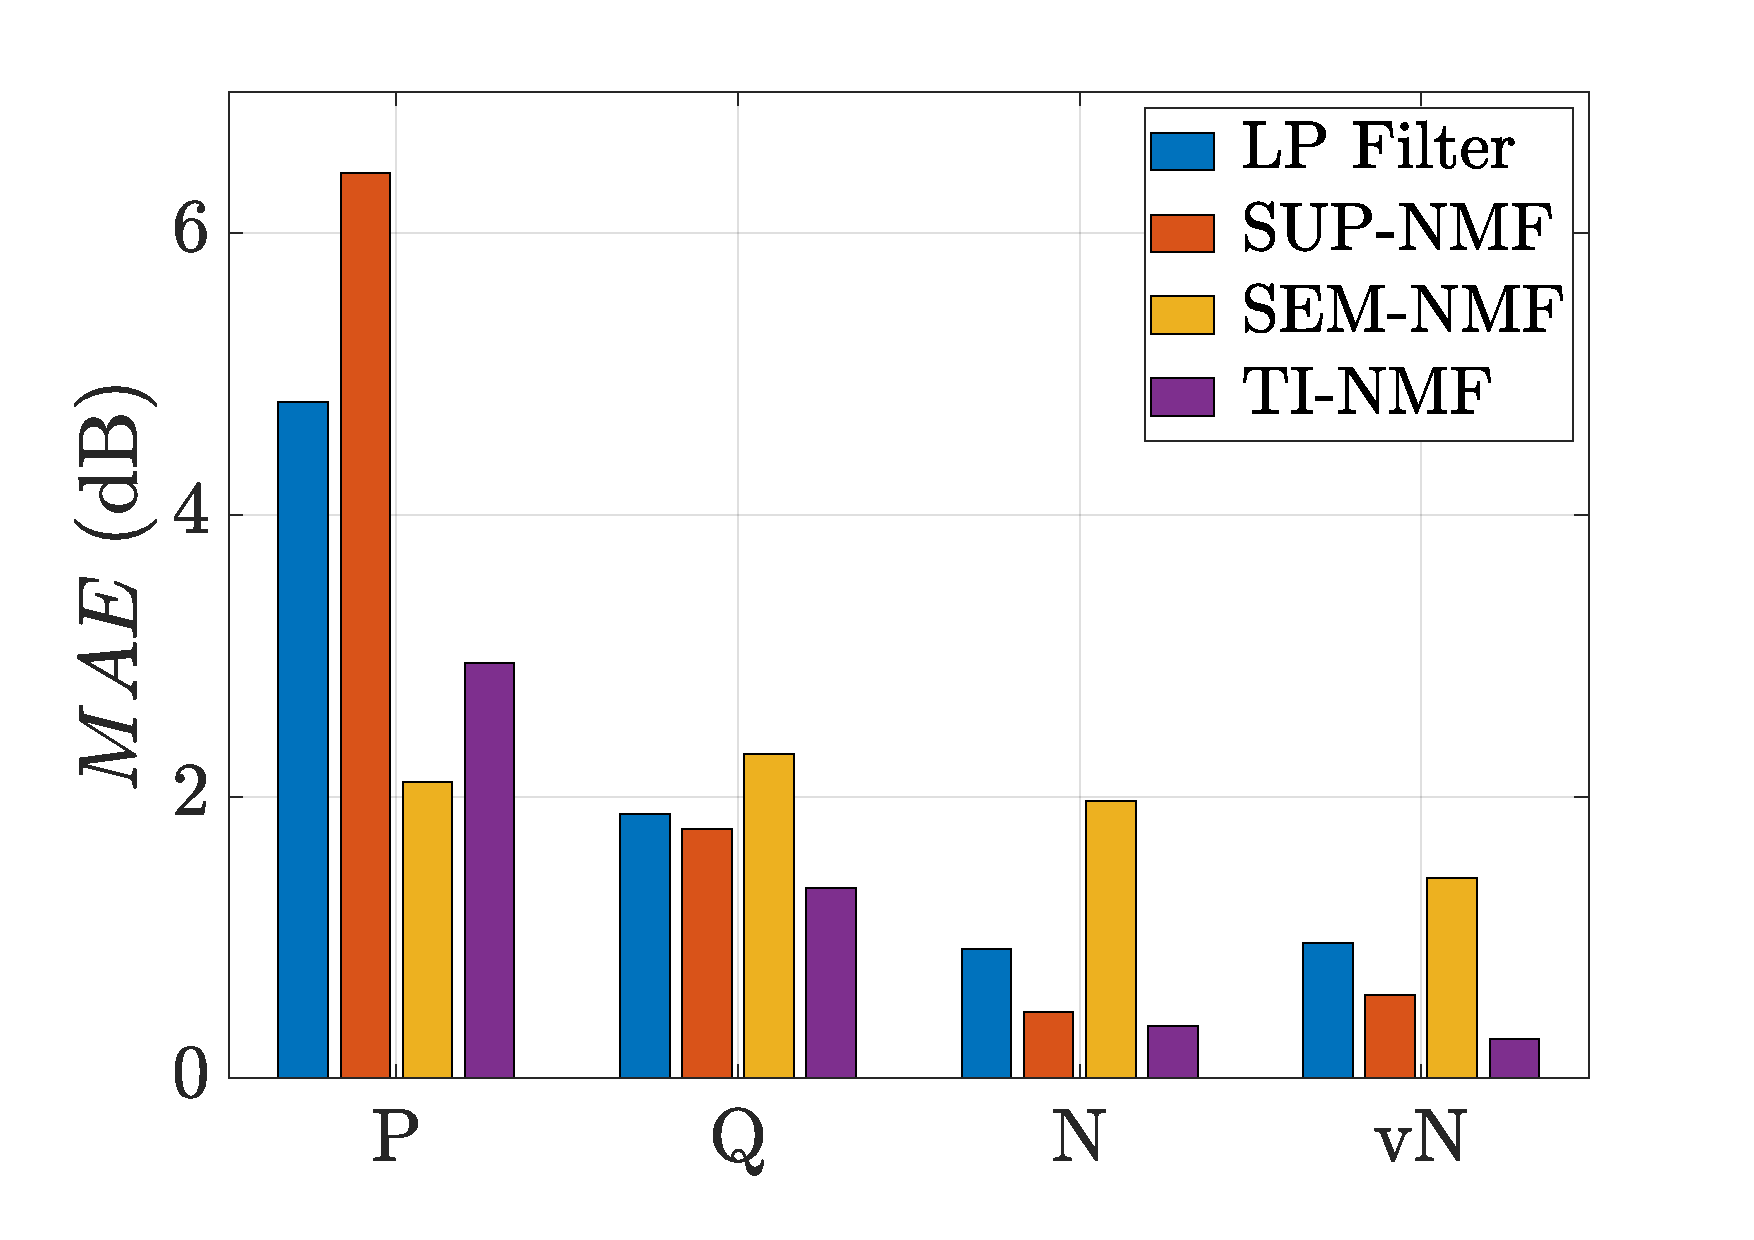
\includegraphics[width=\linewidth]{figures/mea_grafic_bar.pdf}
\caption{$MAE$ errors with the standard deviations according to each sound environment for the best combination of the LP filter ($f_c$ = 500 Hz), SUP-NMF ($\beta$ = 2, $\mathbf{K}$ = 25, $\mathbf{w_t}$ = 1 second), SEM-NMF ($\beta$ = 1, $\mathbf{K}$ = 200, $\mathbf{w_t}$ = 1 second) and TI-NMF ($\beta$ = 2, $\mathbf{K}$ = 200, $\mathbf{w_t}$ = 0.5 second, $\mathbf{t_{h}} = 0.32$).}
\label{fig:mae_env}
\end{figure}

Aside SEM-NMF, all the methods show the same error evolution: a decrease of the error with the increase of the traffic predominance. On contrary, SEM-NMF shows an almost constant error for all 4 sound environments. The LP filter error is mainly important for environments where the traffic is less present. As this approach considers the remaining energy as the traffic component, no distinction is made between the different sound sources not related to the traffic component. The interfering sound class is then wrongly considered as traffic component. On the opposite, for noisy and very noisy environments, the performances of the LP filter are good ($MAE$ $<$ 1 dB). The errors are here due to a high deletion of the traffic energy by the filter while it becomes the main sound source. Consequently, the 500 Hz LP filter estimator provides a low $MAE$ error through the sound environments thank to a balance between the remaining and discarded energy. 

Despite a fixed dictionary composed of traffic spectra, SUP-NMF fails to identify correctly the traffic component particularly for \textit{park} ($MAE$ = 6.42 dB) environments. With this method, as NMF minimizes the cost function, eq. \ref{eq:min-D-WH}, the dictionary's elements are used to model the other sound sources which can not allow a rightful approximation of the traffic component. On the opposite, for \textit{noisy} and \textit{very noisy} environments, SUP-NMF identifies correctly the traffic components ($MAE$ $<$ 0.6 dB) as it is the main source.
In the case of SEM-NMF, adding the mobile dictionary, $\mathbf{W_r}$, makes it possible to include the other sound sources not present in the dictionary. If this behavior is advantageous for the \textit{park} environment ($MAE$ = 2.10 dB) where lot of different kind of sources are present, it is less advantageous for the rest of the environments where the traffic becomes predominant resulting in the highest errors. Indeed, this degree of freedom generates higher error as $\mathbf{W_r}$ is not constrained and is free to include traffic component in it, penalizing the traffic sound level estimation.

Finally, TI-NMF presents the most performing results, except in the \textit{park} environment ($MAE$ = 2.95 dB). In this sound environment, with the threshold value $t_h$ = 0.32, the traffic dictionary is composed, on average, of 136 elements.
By increasing this value, it would be possible to put aside the spectra furthest away of the traffic elements and then decrease the error. For the rest of the sound environments, TI-NMF has the lowest errors. For very noisy environment the error is even very low ($MAE=$ 0.28 dB). With on average 198 elements in $\mathbf{W}_{traffic}$, almost all the elements present in $\mathbf{W'}$ can be considered as traffic elements. 

Considering a unique dictionary fitted to the sound scene under evaluation thus makes TI-NMF very effective when traffic is predominant, while the thresholding step make it possible to discards the elements of the dictionary that deviate too much when the traffic is less present.

\section{Conclusion}

The non-negative matrix factorization framework has been considered as a source separation tool to estimate the traffic sound level  from a corpus of urban sound scenes artificially built. Those scenes are designed to be as similar as possible to the outputs of a deployed sensor networks with the advantages of the simulation process (sound level and position of each source controlled and known). The realism of the scenes has been verified thanks to a perceptual test.

The results confirm the potential of the NMF method on such application scenario as it takes into account the overlap between the multiple sound sources present in cities and is suited to monophonic sensor networks. Different NMF algorithmic schemes have been studied through the supervised and semi-supervised approach. On all the sound environments, these common approaches reveal to be not sufficiently efficient: supervised NMF approach, with its fixed dictionary, does not succeed to estimate correctly the traffic sound level especially when this sound source is quiet, while semi-supervised approach with the presence of a mobile part in the dictionary is the best estimator for \textit{park} environments but fails on heavily traffic scenes.

The proposed approach, named Thresholded Initialized NMF, achieved the lowest error in the evaluation corpus. Consequently, in the case where the location or the type of sound environments the sensors are monitoring cannot be identified (for instance within a mobile measurement framework), TI-NMF appears to be the most appropriate method. If the sound environment can be identified through a prior analysis, or based on positioning data \cite{can2015noise,lavandier2016urban}, it should be possible to adapt the estimation procedure by selecting the most efficient approach in order to further reduce the error in the estimated road traffic sound levels.

Further analyses are required to extend the proposed method to other sound sources, such as birds or voices sounds, which can conveniently be done by replacing or adding elements in the dictionary. This utilization would be useful in the context of muti-source noise mapping that is gaining interest \cite{aumond2017Probabilistic, aletta2015soundscape}. Finally, the parameters selected in this study are valid for this evaluation corpus. Further analyses on various corpus of sound scenes are needed to evaluate the robustness of the method and select the most relevant approaches for specific sound environments (predominance of water or industrial sounds, rural environments \dots).

For reproducibility purposes, the evaluation corpus, the experimental protocol and the programs developed under the Matlab software are available online \footnote{\url{https://github.com/jean-remyGloaguen/articleNmfTrafficSimScene2018}} as the sound dataset \footnote{\url{https://zenodo.org/record/1184443}}. 

\section*{Acknowledgements}
The authors would like to thank Pierre Aumond and Catherine Lavandier from the University of Cergy-Pontoise for transmitting us the data of the \textit{Grafic} project.

\section*{Funding}
This study is co-funded by Ifsttar and Pays de la Loire region.
% with a partial funding from the ANR under project reference ANR-16-CE22-0012.

\section*{References}
\bibliographystyle{elsarticle-num}
\bibliography{bibliographie_applied}

\end{document}
